\chapter{Planned and Preliminary Results}
\label{ch:results}

This chapter is a draft. The terrain and wind extraction, the CR parameter fit on the current cleaned cohorts, and all model training described in Chapter~\ref{ch:methodology} have not been completed at the time of writing. The tables below are placeholders showing the intended reporting format. The figures are examples from an earlier version of the Aberfoyle dataset and workflow, included to show the type of output planned, not as final results.

\section{Trajectory analysis and spatial structure}

\subsection*{Chapman-Richards baseline fit}

Figure~\ref{fig:cr-example} shows the intended output format for the CR baseline: observed height-age trajectories for individual plots plotted against a fitted CR curve. The curve shown uses provisional parameters from an earlier exploratory pass and has not been refitted on the current cleaned four-survey cohort.

\begin{figure}[h]
\centering
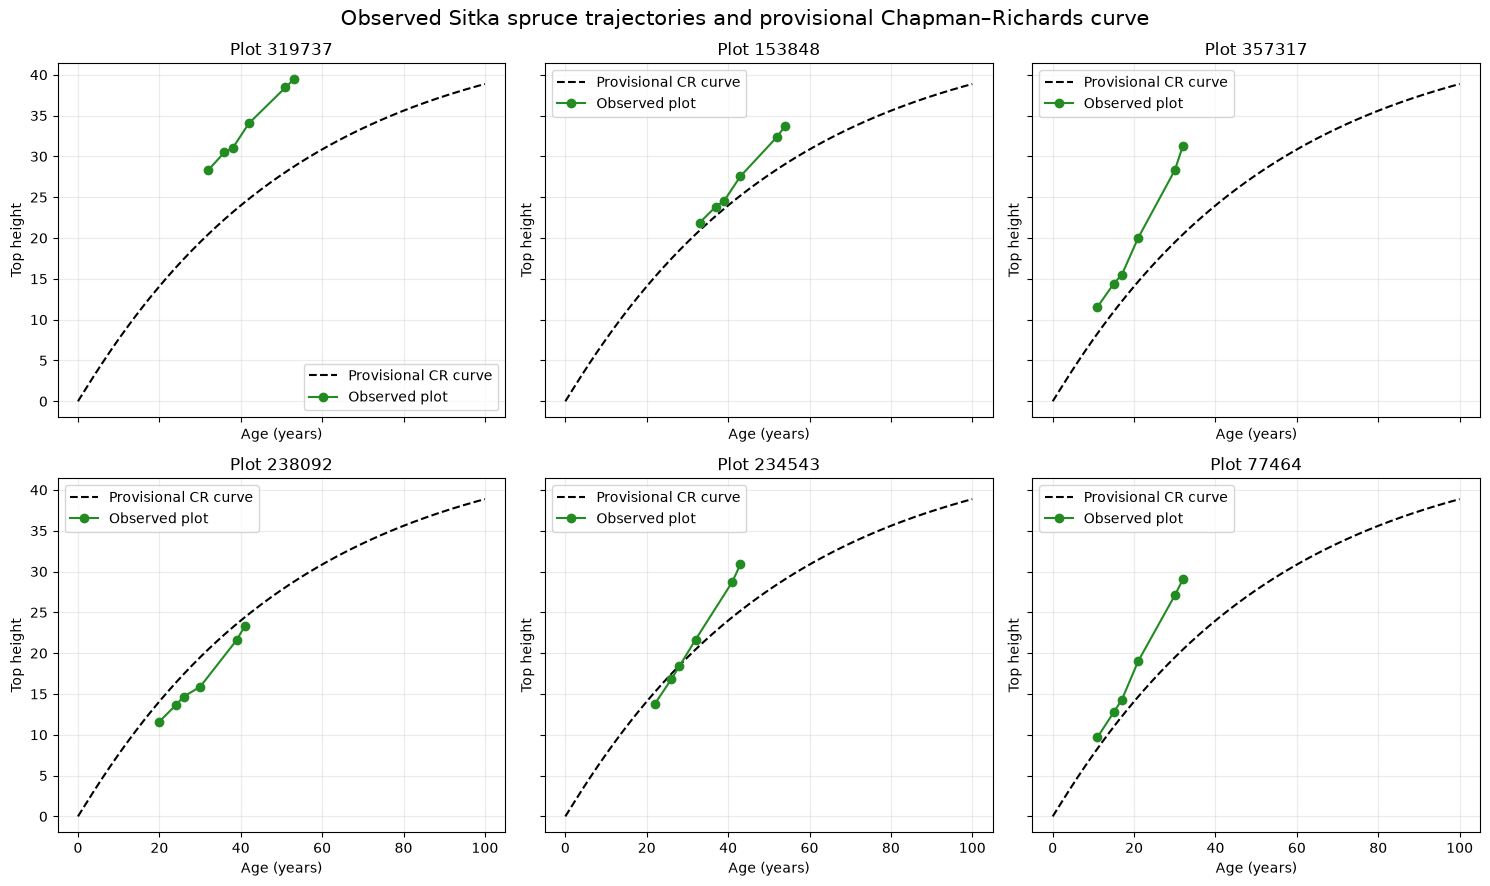
\includegraphics[width=\textwidth]{figures/legacy_examples/cr_trajectories_example.png}
\caption{Example figure from an earlier Aberfoyle dataset/workflow. Included to illustrate the planned analysis; not a final result. Observed Sitka spruce height-age trajectories for six example plots against a provisional Chapman-Richards curve fitted during exploratory analysis on a prior GeoPackage version.}
\label{fig:cr-example}
\end{figure}

\subsection*{Distribution checks by survey year}

Figure~\ref{fig:canopy-example} shows the intended format for checking whether a variable's distribution is stable or shifting across survey years, here for canopy cover on an earlier dataset version. The equivalent check for \texttt{Top\_Height95} on the current cleaned cohorts is outstanding.

\begin{figure}[h]
\centering
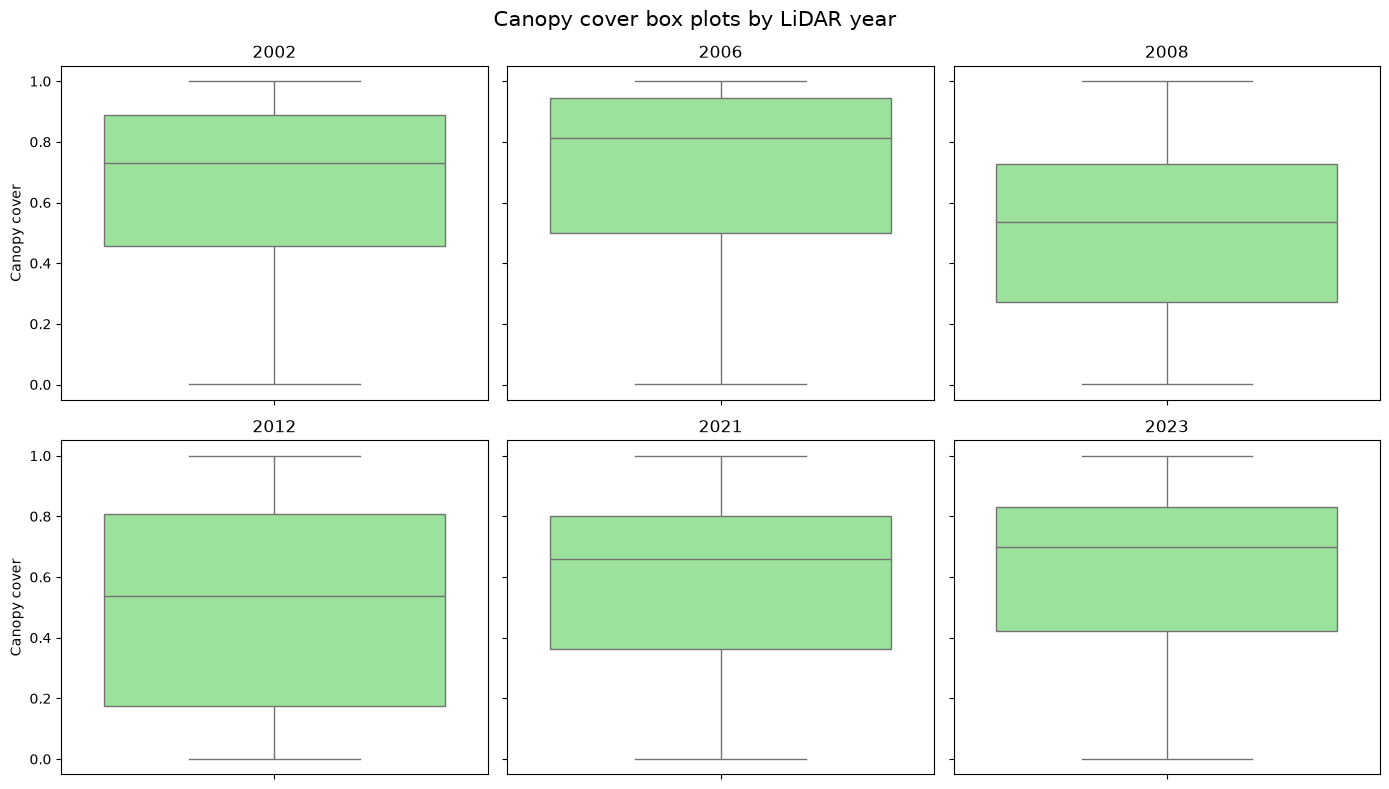
\includegraphics[width=\textwidth]{figures/legacy_examples/canopycover_by_year_example.png}
\caption{Example figure from an earlier Aberfoyle dataset/workflow. Included to illustrate the planned analysis; not a final result. Canopy cover box plots by LiDAR survey year, from an earlier exploratory pass on a prior GeoPackage version.}
\label{fig:canopy-example}
\end{figure}

\subsection*{Moran's I and trajectory classes}

\begin{table}[h]
\centering
\begin{tabular}{lc}
\toprule
Statistic & Value \\
\midrule
Global Moran's I on $\bar{\varepsilon}_i$ & TODO \\
$p$-value & TODO \\
Number of LISA high-high clusters & TODO \\
Number of LISA low-low clusters & TODO \\
\bottomrule
\end{tabular}
\caption{Placeholder: Moran's I and LISA results, not yet computed on the current cleaned cohort.}
\label{tab:moran-placeholder}
\end{table}

\section{Spatial attribution: XGBoost and SHAP}

\begin{table}[h]
\centering
\begin{tabular}{lccc}
\toprule
Model & RMSE & R\textsuperscript{2} & Top 3 SHAP features \\
\midrule
XGB-A (terrain only) & TODO & TODO & TODO \\
XGB-B (terrain + wind) & TODO & TODO & TODO \\
\bottomrule
\end{tabular}
\caption{Placeholder: XGBoost attribution results, pending terrain and wind feature extraction.}
\label{tab:xgb-placeholder}
\end{table}

\section{Env-PINN results}

\begin{table}[h]
\centering
\begin{tabular}{lccccc}
\toprule
Model & MAE & MSE & R\textsuperscript{2} & MRE & Accuracy \\
\midrule
CR (global parameters) & & & & & \\
Linear regression & & & & & \\
XGB-B (terrain + wind) & & & & & \\
PINN v1 (baseline, global $y_{\max}$) & & & & & \\
Env-PINN v2 (terrain-conditioned) & & & & & \\
Env-PINN v3 (full-conditioned) & & & & & \\
\bottomrule
\end{tabular}
\caption{Placeholder: model comparison table. To be reported separately for all plots, persistent under-performers, and CR-conformant plots once training is complete.}
\label{tab:model-comparison-placeholder}
\end{table}

\section{Synthesis (placeholder)}

Once the above results exist, this section will report what fraction of between-plot growth variation terrain and wind features explain (from the XGB-B $R^2$), whether Moran's I on the XGBoost residuals drops relative to Moran's I on the raw CR residuals (a check on whether the features genuinely capture spatial structure rather than simply proximity), and what fraction of variation remains unexplained -- expected, based on the data audit in Chapter~\ref{ch:data}, to include a contribution from unrecorded thinning and management events.
